\begin{figure}[H]
\centering
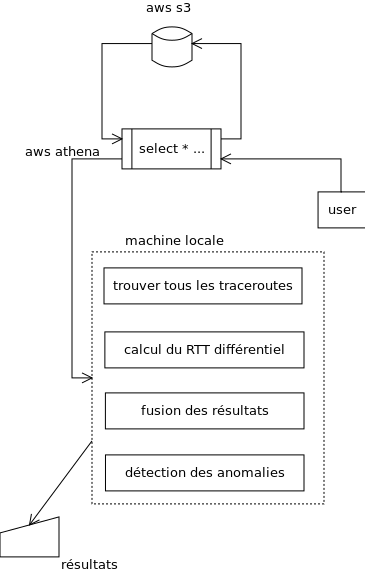
\includegraphics[width=1\linewidth]{illustrations/scenarios-before-after}
\caption{}
\label{fig:scenarios-before-after}
\end{figure}

\begin{figure}[H]
\centering
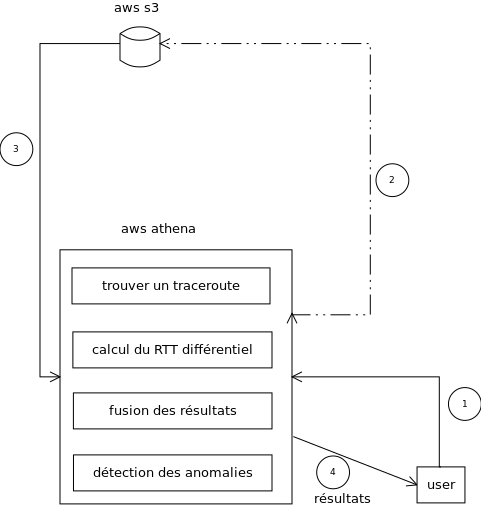
\includegraphics[width=1\linewidth]{illustrations/tentative-athena-all}
\caption{}
\label{fig:tentative-athena-all}
\end{figure}


  		\State $ traceroutes  \leftarrow  findTraceroutes(currDate) $
  		\ForAll {$trace \in traceroutes$}
  		readOneTraceroute()
  		\EndFor
  		
  		\begin{table}[H]
  			\resizebox{\textwidth}{!}{
  				\begin{tabular}{c c c c}
  					(IP1,IP2)&	RTT	&Probes&	MSM \\
  					('185.147.12.31', '185.147.12.19') &	[-0.02900000000000036]&	['89.105.202.4']&	
  					
  					5004 : set([4247]) \\
  					
  					('196.216.164.1', '196.12.10.246')&	[-1.379]&	['196.216.164.50']	&
  					
  					5004 : set([14465]) \\
  					
  					('185.147.12.19', '160.242.100.88')&	[0.5350000000000001]&	['89.105.202.4']	&
  					
  					5004 : set([4247]) \\
  					
  					('196.12.10.246', '160.242.100.88')&	[0.21799999999999997]&	['196.216.164.50']	&
  					
  					5004 : set([14465]) \\
  					
  					('196.49.6.10', '192.5.5.241')&	[3.4729999999999848]&	['196.216.164.50']	&
  					
  					5004 : set([14465]) \\
  					
  					('89.105.200.57', '185.147.12.31')&	[1.463]&	['89.105.202.4']	&
  					
  					5004 : set([4247]) \\
  					
  					('196.216.48.144', '193.239.116.112')&	[1.6290000000000004]&	['89.105.202.4']	&
  					
  					5004 : set([4247]) \\
  					
  					('193.239.116.112', '192.5.5.241')&	[0.5169999999999995]&	['89.105.202.4']&	
  					
  					5004 : set([4247]) \\
  					
  					('160.242.100.88', '196.216.48.144')&	[63.474000000000004, 2.404]&	['196.216.164.50', '89.105.202.4']&	
  					
  					5004 : set([14465, 4247]) \\
  				\end{tabular}
  			}
  		\end{table}
  		
  		\begin{algorithm}
  			\caption{calcul des alarmes  }
  			\begin{algorithmic}[1]
  				\Function{outlierDetection}{sampleDistributions}
  				\State d
  				\EndFunction
  			\end{algorithmic}
  			\label{algo:step-alarmsDetection}
  		\end{algorithm}
  		
  		\subsection{Récapitulatif  des résultats I et II}
  		
  		\begin{table}
  			
  			\begin{tabularx}{}{ l c c}
  				\hline
  				&\textbf{Résultat I}& \textbf{Résultat II} \\
  				Principe de la détection &  &\\
  				Paramètres de l'analyse sauf la période &Personnalisables& prédéfinis\\
  				Etapes principales & Récupération des traceroutes et détection&Préparation, ensuite détection\\
  				
  			\end{tabularx}
  		\end{table}